\documentclass[notheorems, 10pt]{beamer}
\usepackage{SlideStyle}
\renewcommand{\epsilon}{\varepsilon}
\usepackage{graphicx}


\titlegraphic{\vspace*{-7cm}
    \parbox[c]{3cm}{
\includegraphics[height=.7cm]{bsulogo}}
    \hspace*{1cm}%
    \parbox[c]{2cm}{
\includegraphics[height=0.6cm]{FPMIlogo_new}}
    \hspace*{1cm}%
    \vspace*{3cm}
}

\title[Модели по данным разной частоты]{\Large Краткосрочное прогнозирование и наукастинг макроэкономических временных рядов на основе векторных моделей авторегрессии по смешанным данным}


\author[Т. А. Бовт]{Бовт Тимофей Анатольевич}

\institute[]{Научный руководитель: В.И. Малюгин}


\date[]{}%{\scriptsize \structure{2017-2018}}


\begin{document}

\begin{frame}[plain]
  \titlepage
\end{frame}


%--------------------------------------------------------------------------------------
\begin{frame}{Основные понятия ВР}
	\begin{itemize}
		\item временные ряды;
		\item стационарность временных рядов;
		\item TS-ряды, понятие тренда;
		\item DS-ряды, единичный корень;
		\item тесты стационарности: DF, ADF;
		\item сезонность;
		\item сезонная корректировка: TRAMO SEAT.
	\end{itemize}
\end{frame}

%--------------------------------------------------------------------------

\begin{frame}
	{Исходные данные}
	Для проведения исследований нам даны следующие экономические показатели
	\begin{itemize}
		\item GDP — ВВП Беларуси по источникам использования доходов в среднегодовых ценах 2018 г. на квартальной частоте;
		\item IPV — объём промышленного производства в среднегодовых ценах 2018
		г. на месячной частоте;
		\item RTV — объём розничного товарооборота в среднегодовых ценах 1995 г.
		на месячной частоте;
		\item BIV — базисный индекс объёма строительно монтажных работ на месячной частоте;
		\item ICV — объём инвестиций в основной капитал в среднегодовых ценах 2018
		г. на месячной частоте;
		\item BIVMP — базисный индекс объёма денежных доходов населения на месячной частоте;
		\item APV — объём продукции сельского хозяйства в среднегодовых ценах 2018
		г. на месячной частоте [5].
	\end{itemize}
	
	Период наблюдения данных следующий
	\begin{itemize}
		\item для квартальных: 1 квартал 2009 года — 2 квартал 2024 года;
		\item для месячных: 1 месяц 2009 года — 6 месяц 2024 года.
	\end{itemize}
\end{frame}
%--------------------------------------------------------------------------
\begin{frame}
	\frametitle{Сезонная корректировка данных}
	$$
		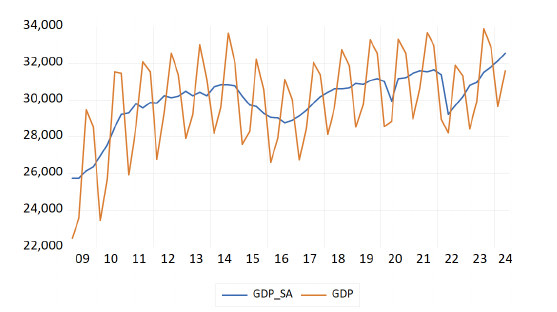
\includegraphics[scale=0.25]{screenshot001}
	$$
	$$
		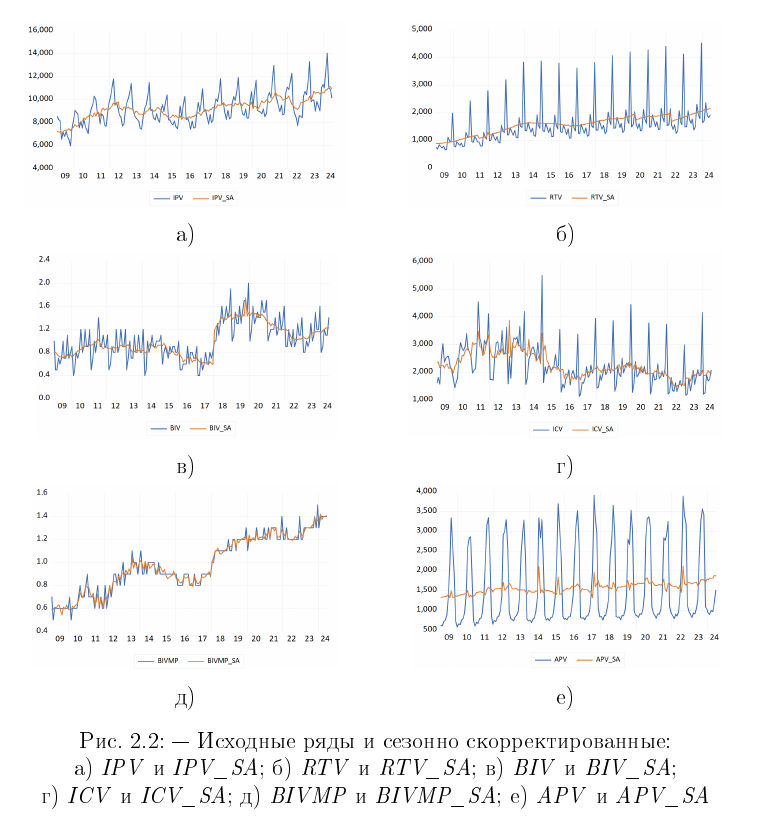
\includegraphics[scale=0.25]{screenshot002}
	$$
	
	
\end{frame}
%--------------------------------------------------------------------------
\begin{frame}
	\frametitle{Исключение тренда}
	$$
		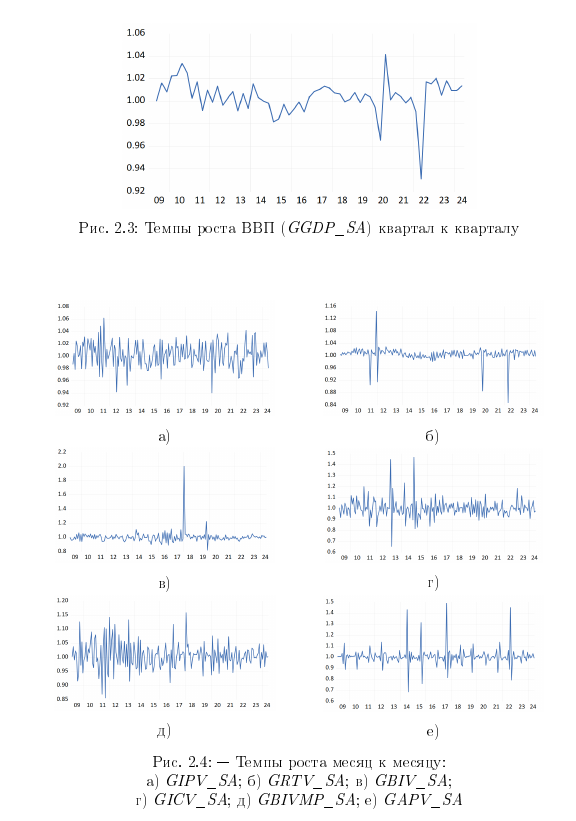
\includegraphics[scale=0.35]{screenshot003}
	$$
	
\end{frame}

\begin{frame}
	\frametitle{ADF тест}
	$$
	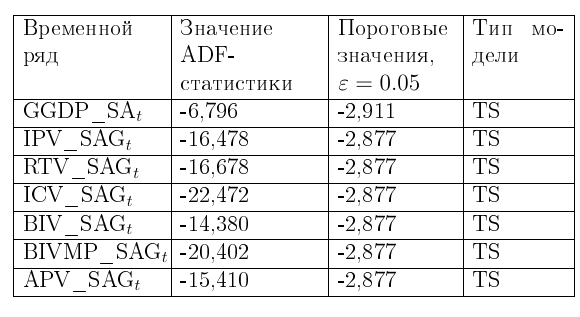
\includegraphics[scale=0.7]{screenshot004}
$$
\end{frame}
%--------------------------------------------------------------------------
\begin{frame}
	\frametitle{MFVAR}
	$$
		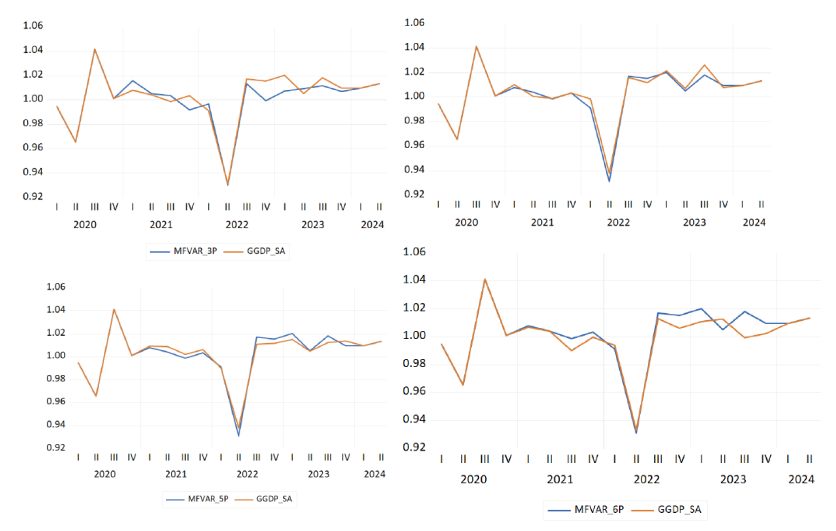
\includegraphics[scale=0.5]{screenshot005}
	$$
	
\end{frame}

%--------------------------------------------------------------------------

\begin{frame}
	\frametitle{Оценки}
	$$
		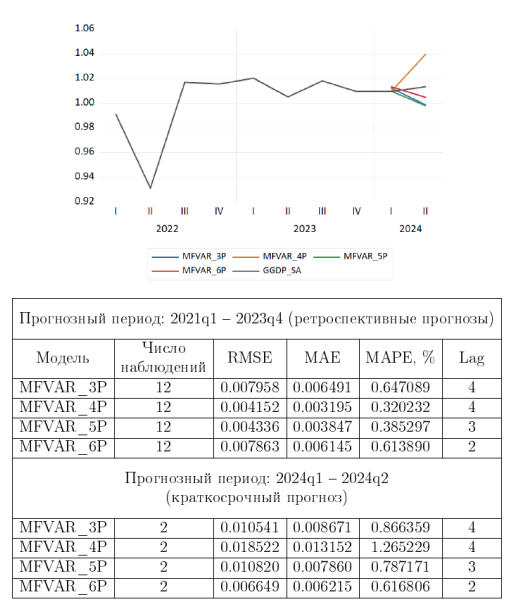
\includegraphics[scale=0.45]{screenshot006}
	$$
	
\end{frame}


%--------------------------------------------------------------------------

\begin{frame}
	{Заключение}
	В данной работе была рассмотрена задача прогнозирования компонент ВВП на основе регрессионных моделей MFVAR. В ходе исследования
	\begin{enumerate}
		\item было дано теоретическое описание всех используемых для решения данной задачи моделей;
		\item были рассмотрены свойства и особенности, которые возникают в ходе работы с исследуемыми моделями;
		\item был проведен полный цикл исследования и преобразования моделей временных рядов для приведения к стационарному виду;
		\item были построены модели MFVAR для прогнозирования и оценки темпов роста ВВП Беларуси по его компонентам, такиим как объем промышленности, объем товарооборота, сельского хозяйства, объем строительства, объем инвестиций, объем доходов населения;
		\item был проведен сравнительный анализ точности прогнозных значений и ретроспективных прогнозов моделей MFVAR в зависимости от переменных.
	\end{enumerate}
\end{frame}

%--------------------------------------------------------------------------

\begin{frame}
	{Используемые источники}
	\begin{enumerate}
	\item Foroni, C. A survey of econometric methods for mixed frequency data / C. Foroni, M. Marcellino // Working Paper 2013/06, Norges Bank.
	\item Ghysels, E., Santa-Clara P., Valkanov R. 2002. The MIDAS touch: Mixed data sampling regression models, Working paper, UNC and UCLA.
	\item Макеева, Н.М., Наукастинг элементов использования ВВП России / Н.М. Макеева, И.П. Станкевич // Статья 2022/10, Экономический журнал ВШЭ.
	\item Foroni, C. Unrestricted Mixed Data Sampling (U-MIDAS): MIDAS Regressions With Unrestricted Lag Polynomials / C. Foroni, M. Marcellino, C. Schumacher // Discussion paper 2015, Deutsche Bundesbank.
	\item Станкевич И.П. Сравнение методов наукастинга макроэкономических индикаторов на примере российского ВВП // Прикладная эконометрика 2020. С. 113–127.
	\item Харин, Ю. С. Теория вероятностей, математическая и прикладная статистика / Ю. С. Харин, Н. М. Зуев, Е. Е. Жук // Минск : БГУ, 2011. 
	\end{enumerate}
\end{frame}

\end{document} 